\setcounter{page}{1}

\section{Objetivos}
    \begin{itemize}
        \item Diseñar e implementar una red de acuerdo con los requerimientos de un instituto educativo
    \end{itemize}

\section{Introducción}

El diseño de redes es una de las áreas fundamentales dentro del ámbito de las tecnologías de la información, ya que permite conectar de manera eficiente los dispositivos y sistemas de una organización. En este proyecto, se busca diseñar y simular la infraestructura de red para el instituto “Ing. Fátima Montserrat”, teniendo en cuenta las necesidades específicas de sus principales usuarios: Profesores, Alumnos y Administrativos. Este diseño tiene como objetivo principal garantizar una comunicación fluida, segura y escalable entre los diferentes departamentos.

La dirección IP asignada para el desarrollo de la red es \texttt{192.168.10.0/24}. A partir de este rango, se utilizarán técnicas de subnetting para dividir la red en subredes más pequeñas y manejables. Este proceso es clave para optimizar el uso de direcciones IP, ya que cada subred permitirá segmentar el tráfico y reducir la congestión en la red principal. Adicionalmente, se implementarán VLANs para separar lógicamente el tráfico de cada grupo de usuarios, reforzando la seguridad y mejorando el rendimiento de la red.

El desarrollo del proyecto incluye varios pasos. En primer lugar, se realizará el cálculo de las subredes necesarias para cubrir los requerimientos del instituto, identificando la dirección de red, la dirección de broadcast y el rango de direcciones disponibles para cada subred. Posteriormente, se procederá a la configuración lógica de la red, asignando puertos específicos a cada subred y asegurando que la topología sea sencilla de administrar y mantener. Además, se integrarán servicios básicos como servidores DNS y web, necesarios para el funcionamiento de la red.

Finalmente, se realizará una simulación del diseño propuesto en un entorno virtual, con el fin de verificar su funcionalidad y realizar ajustes antes de su implementación real. Este proceso es crucial para identificar posibles fallos y optimizar el diseño de la red. Al concluir el proyecto, se analizarán los resultados obtenidos y se evaluará la eficiencia del diseño en términos de uso de recursos, seguridad, rendimiento y escalabilidad.


\section{Problemática}
El instituto ``Ing. Fátima Montserrat'' requiere la comunicación, vía red, para miembros de su comunidad de acuerdo con intereses comunes.
Para ello, cuenta con la IP \texttt{192.168.10.0/24} para atender a 3 conjuntos:
    \begin{itemize}
        \item Profesores
        \item Alumnos
        \item Administrativos
    \end{itemize}

Por ahora, cada conjunto contará solo con 2 computadoras y un servidor web distribuidos en 3 pisos: un equipo por piso. A raíz de un análisis previo se propone el empleo de un switch por nivel y estarían enlazados por medio de otro switch ubicado en el nivel 1, como se muestra en la figura \ref{fig:topologia}.

\begin{figure}[H]
    \centering
    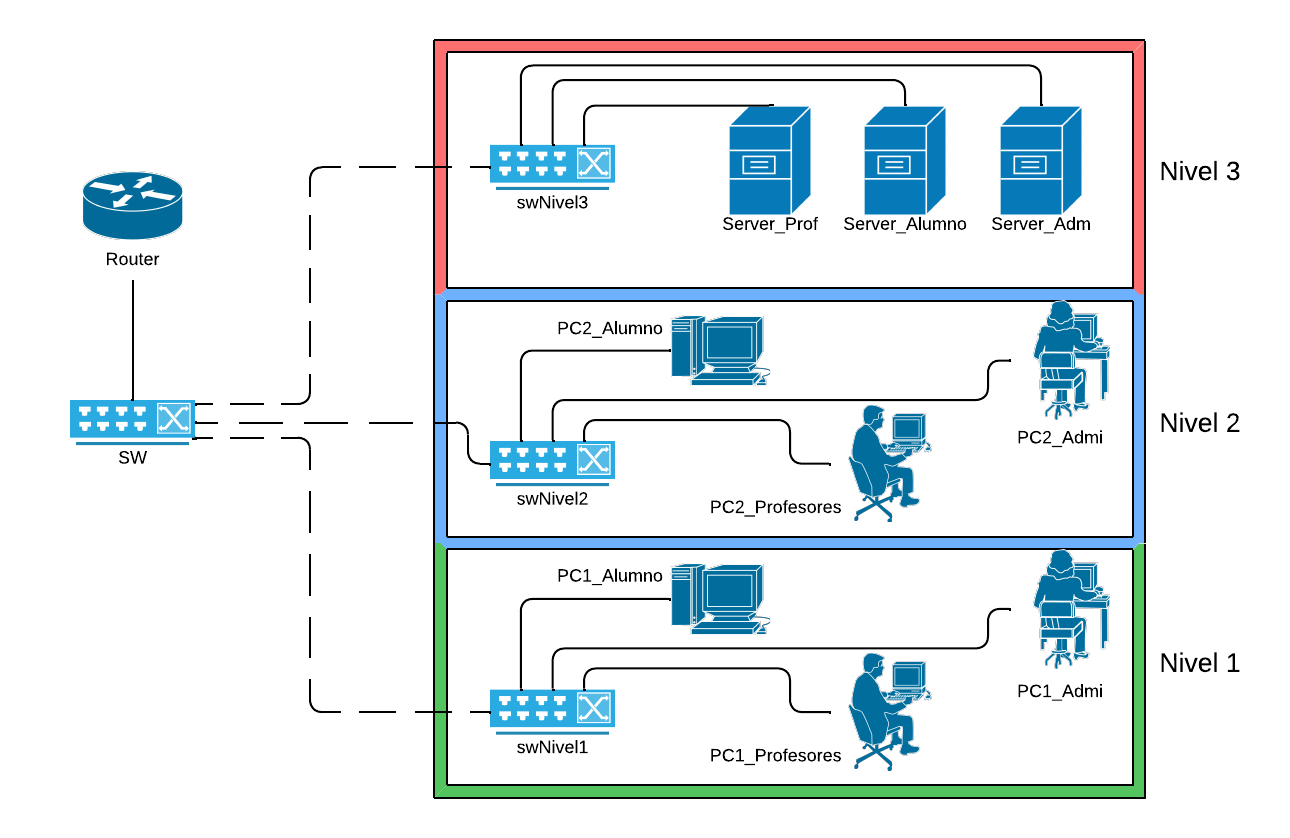
\includegraphics[width=0.6\textwidth]{img/topologia.png}
    \caption{Topología de la red}
    \label{fig:topologia}
\end{figure}

Los switches sugeridos por el consejo técnico del Instituto son cuatro serie 2960 de cisco modelo Ws-c2960 24lc-s y el router Serie 2900.

La asignación de puertos, de acuerdo con los requerimientos, es la siguiente:

\begin{enumerate}
    \item Puerto 1 a 7 para Profesores
    \item Puerto 8 a 15 para Alumnos
    \item Puerto 16 a 23 para Administrativos
\end{enumerate}

Además, durante el diseño se debe contemplar lo siguiente:

\begin{enumerate}
    \item [1] Proponga e implemente el diseño de la solución a este requerimiento en el simulador.
    \item [2] Realice la cotización del material y equipo a emplear. Recuerde que el Instituto ya cuenta con los equipos de cómputo.
    \item [3] Realice los planos de distribución (vista aérea y vista lateral).
\end{enumerate}

\section{Desarrollo del Trabajo}

    \subsection{Cálculo de Subredes}

    Para comenzar con el diseño de la red, se debe obtner las subredes necesarias para la red del instituto. Para ello, se debe calcular la cantidad de bits necesarios para la cantidad de dispositivos que se tienen en cada subred.

    \subsubsection*{Paso 1: Calcular la cantidad de subredes necesarias}

    Para el cálculo de las subredes necesarias, se deben considerar los siguientes aspectos:
    \begin{itemize}
        \item El número total de subredes requeridas.
        \item En este caso, utilizaremos 3 subredes (Profesores, Alumnos y Administrativos). Sin embargo, dado que no se suele usar la primera subred en ciertas prácticas, se necesitarán 4 subredes en total
    \end{itemize}
    Para calcular el número de subredes necesarias, utilizamos la siguiente fórmula:

    \begin{equation} 
        2^{n} \geq \text{Número de subredes requeridas} 
    \label{eq:subredes} 
    \end{equation}
    Indicamos el indice necesario para la cantidad de subredes:
    \begin{equation} 
        n = 2 \label{eq:nsub} 
    \end{equation}
    De acuerdo con la ecuación, tenemos que:
    \begin{equation} 
        2^{4} \geq 4 \label{eq:numeroseb} 
    \end{equation}

    \subsubsection*{Paso 2: Calcular el rango de direcciones IP}

    Para calcular el rango de direcciones, primero debemos determinar la máscara de subred. En nuestro ejemplo, la máscara es \textbf{255.255.255.0}lo que implica que los primeros 24 bits (o tres octetos) están destinados a la parte de la red, y el último octeto está disponible para las direcciones de host.

    Utilizando el valor de \textbf{n} obtenido previamente, que es el número de bits que se van a usar para las subredes adicionales, podemos determinar que se utilizarán 2 bits adicionales en la máscara de red para subdividir las subredes.
    
    Esto nos lleva a modificar la máscara original, ampliando el número de bits reservados para la red. La asignación de los bits de la máscara de red queda de la siguiente manera:
    
    \begin{equation} 
        1111 1111.1111 1111.1111 1111.1100 0000 
    \end{equation}
    
    Al convertir esta representación binaria a formato decimal, obtenemos el valor \textbf{192}. Este valor nos indica cuántas direcciones de host están disponibles en cada subred.
    
    Para calcular el rango de direcciones de cada subred, debemos restar este valor de 256, ya que el valor máximo de una dirección en un octeto es 255, y necesitamos conocer cuántas direcciones quedan disponibles para asignar a los hosts dentro de cada subred. Realizamos la siguiente operación:
    
    \begin{equation} 
        256 - 192 = 64 
    \end{equation}
    
    Esto significa que cada subred tendrá un bloque de 64 direcciones disponibles. De esta manera, obtenemos el rango de direcciones para cada subred, lo cual es crucial para la asignación de direcciones IP en la red.

    \subsubsection*{Paso 3: Obtener la IP de red y la IP de broadcast}

    \begin{table}[H]
        \begin{center}
            \begin{tabular}{ c | c | c | c | c }
                \textbf{Subred} & \textbf{VLAN} & \textbf{IP de Red} & \textbf{Broadcast} & \textbf{Puerto}\\ \hline
                1 & - & 192.168.10.0 & 192.168.10.63 & - \\
                2 & Profesores & 192.168.10.64 & 192.168.10.127 & 1 al 7\\
                3 & Alumnos & 192.168.10.128 & 192.168.10.191 & 8 al 15\\
                4 & Administrativos & 192.168.10.192 & 192.168.10.255 & 16 al 23\\
            \end{tabular}
            \caption{Subredes y VLANs}
            \label{tab:VLANs}
        \end{center}
    \end{table}

    \subsubsection*{Paso 4: Calcular la cantidad de hosts por subred}
    Para calcular el número de hosts disponibles en cada subred, utilizamos la siguiente fórmula:
    \begin{equation}
        \text{Número de hosts por subred} = 2^h - 2
        \label{eq:hosts}
    \end{equation}

    Donde \textbf{h} representa el número de bits disponibles para los hosts en cada subred. Restamos 2 para excluir las direcciones reservadas para la red y el broadcast.
    
    En este caso, la máscara de subred es \textbf{/26}, lo que significa que se han reservado 26 bits para la red, dejando \( 32 - 26 = 6 \) bits para los hosts. Sustituyendo este valor en la ecuación \ref{eq:hosts}:
    
    \begin{equation}
        \text{Número de hosts por subred} = 2^6 - 2 = 64 - 2 = 62
    \end{equation}
    
    Por lo tanto, cada subred puede tener un máximo de \textbf{62} hosts disponibles.

    \subsection{Simulación del proyecto}
    \subsection*{Asignación de las IPs para cada servicio}

    En la siguinte tabla se mostraran las ip de cada uno de los servicios necesarios para esta practica.

    \begin{table}[H]
        \begin{center}
            \begin{tabular}{ c | c | c | c | c }
                \textbf{Subred} & \textbf{VLAN} & \textbf{IP Servidor web/DNS} & \textbf{Ip DHCP} & \textbf{IP gateway}\\ \hline
                1 & Profesores & 192.168.10.126 & 192.168.10.64 & 192.168.10.65\\
                2 & Alumnos & 192.168.10.190 & 192.168.10.128 & 192.168.10.129\\
                3 & Administrativos & 192.168.10.254 & 192.168.10.192 & 192.168.10.193\\
            \end{tabular}
            \caption{IPs para cada servicio}
            \label{tab:redes}
        \end{center}
    \end{table}


    \subsection*{Diseño del modelo en el simulador}
    Para este modelo se solicitó la siguiente topología basada en la presentada anteriormente:
    
    \begin{figure}[H]
        \centering
        \includegraphics[width=0.6\textwidth]{img/diseñoSimulador.png}
        \caption{Diseño de la red en el simulador}
        \label{fig:disSim}
    \end{figure}
    
    \subsection*{Asignación de IPs en los servidores Web}
    Para esta asignación utilizaremos el cuadro 2, el cual nos mostrará las IP requeridas, de forma que la asignación de IP en los servidores quedaría de la siguiente forma:
    
    \begin{figure}[H]
        \centering
        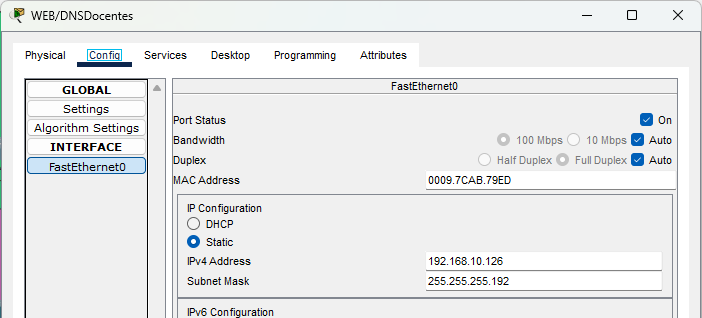
\includegraphics[width=0.7\textwidth]{img/serverprofesores.png}
        \caption{Asignación de IPs en el servidor Web de Profesores}
        \label{fig:serIP}
    \end{figure}
    \begin{figure}[H]
        \centering
        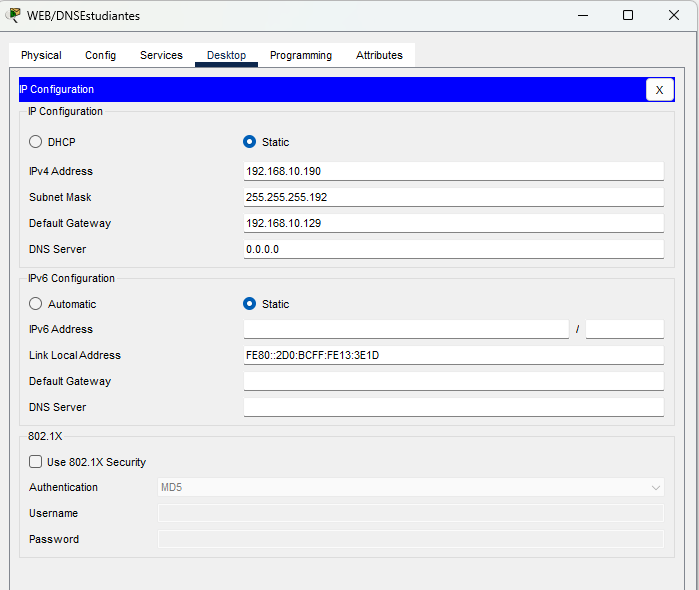
\includegraphics[width=0.7\textwidth]{img/serverestudiantes.png}
        \caption{Asignación de IPs en el servidor Web de Estudiantes}
        \label{fig:seresIP}
    \end{figure}
    \begin{figure}[H]
        \centering
        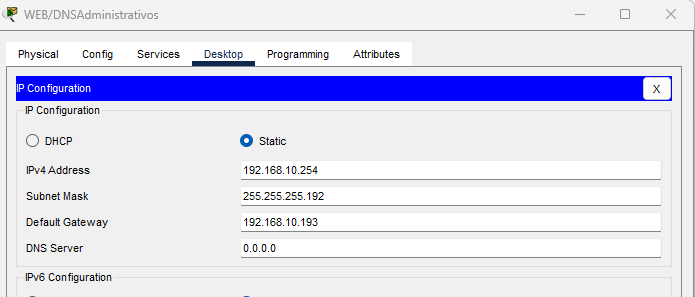
\includegraphics[width=0.7\textwidth]{img/serveradmin.png}
        \caption{Asignación de IPs en el servidor Web de Administrativos}
        \label{fig:seradIP}
    \end{figure}

    \subsection*{Asignación del DNS en los servidores Web}
    Para la asignación de DNS, utilizaremos las direcciones IP que se encuentran en el cuadro 2. Además, esta configuración se aplicará a todos los servidores, de manera que la asignación del DNS en los servidores quedaría de la siguiente forma:
    \begin{figure}[H]
        \centering
        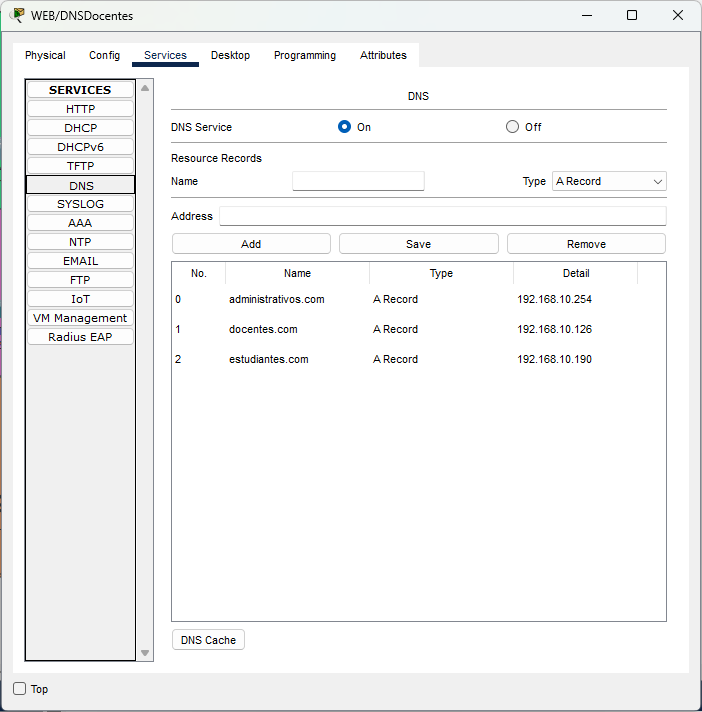
\includegraphics[width=0.7\textwidth]{img/dns.png}
        \caption{Asignación de DNS en todos los servidores Web}
        \label{fig:dns}
    \end{figure}

    \subsection*{Configuración de las VLANs}
    Para la practica utilizaremos los puertos asignados para cada una de las VLANs en cada uno de los switch, de esta forma:
    
    \begin{figure}[H]
        \centering
        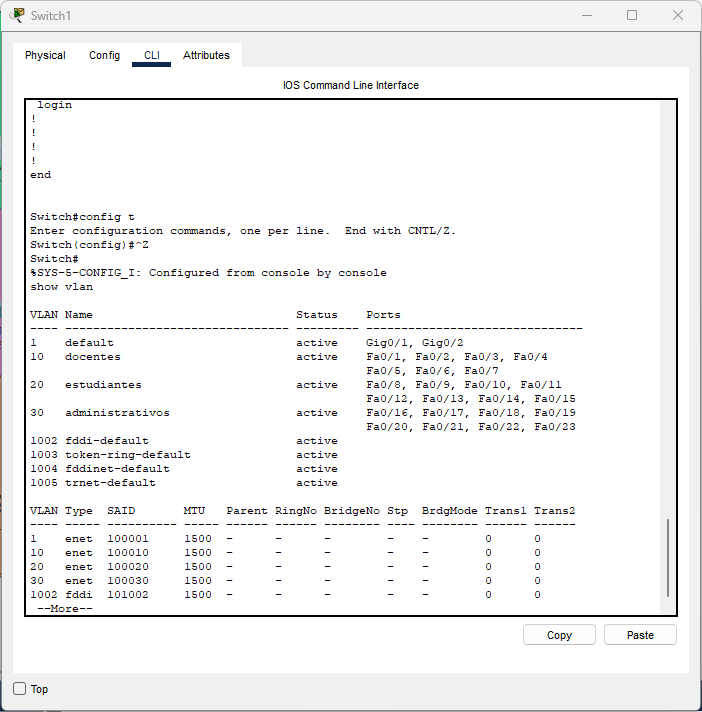
\includegraphics[width=0.6\textwidth]{img/switch1vlan.png}
        \caption{Asignación de puestos en las VLANs Switch 1}
        \label{fig:swvla1}
    \end{figure}
    \begin{figure}[H]
        \centering
        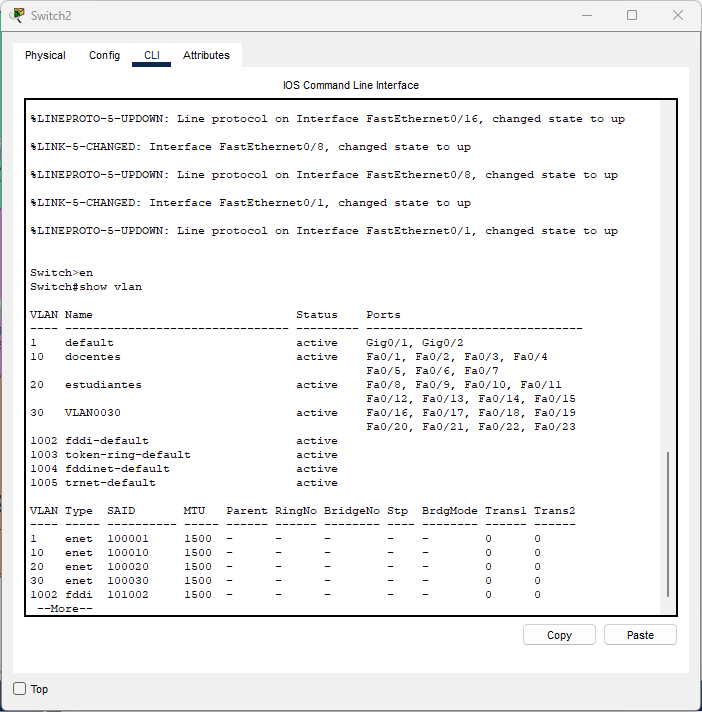
\includegraphics[width=0.6\textwidth]{img/swtichvlan2.png}
        \caption{Asignación de puestos en las VLANs Switch 2}
        \label{fig:swvla2}
    \end{figure}
    \begin{figure}[H]
        \centering
        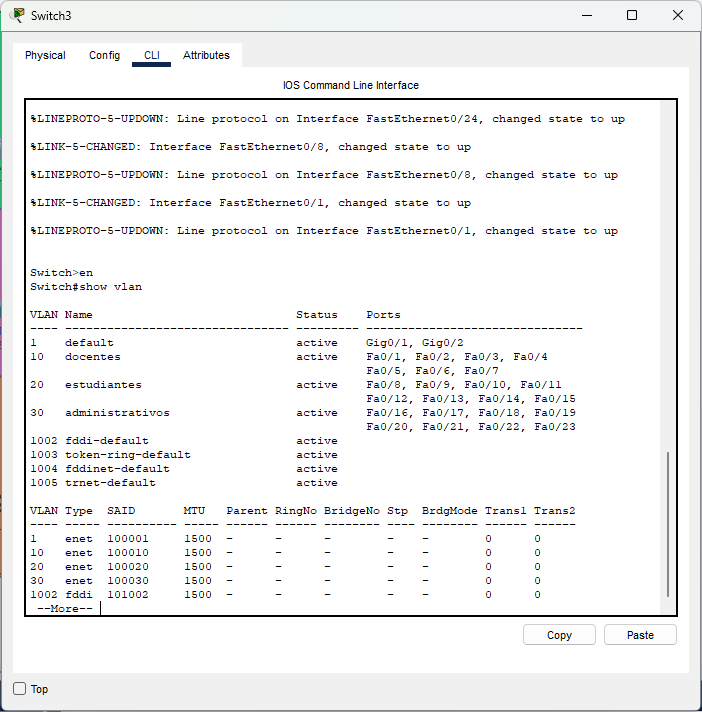
\includegraphics[width=0.6\textwidth]{img/switchvlan3.png}
        \caption{Asignación de puestos en las VLANs Switch 3}
        \label{fig:swvla3}
    \end{figure}
    En esta imagen se puede observar que no tinen puertos asignados y esto es para que se haga efectivo el manejo del trunk.
    \begin{figure}[H]
        \centering
        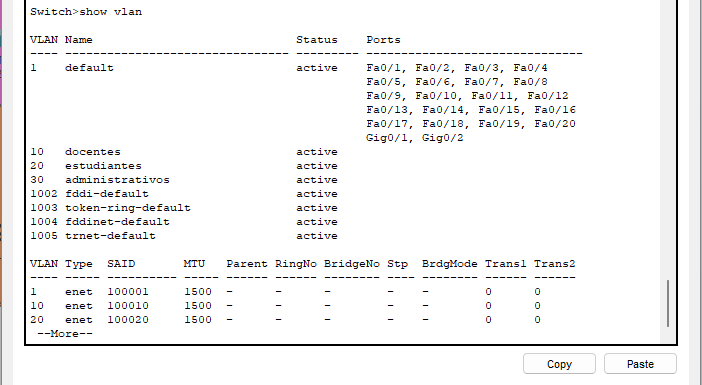
\includegraphics[width=0.6\textwidth]{img/vlansw4.png}
        \caption{Asignación de las VLANs Switch 4}
        \label{fig:swvla4}
    \end{figure}
    \subsection*{Configuración de los trunk en las VLANs}
    La práctica indica la comunicación efectiva entre los switchs por lo que es esencial un buen manejo de los trunk, de forma que los 4 dispositivos deben ser configutados de forma que quede asi:
    
    \begin{figure}[H]
        \centering
        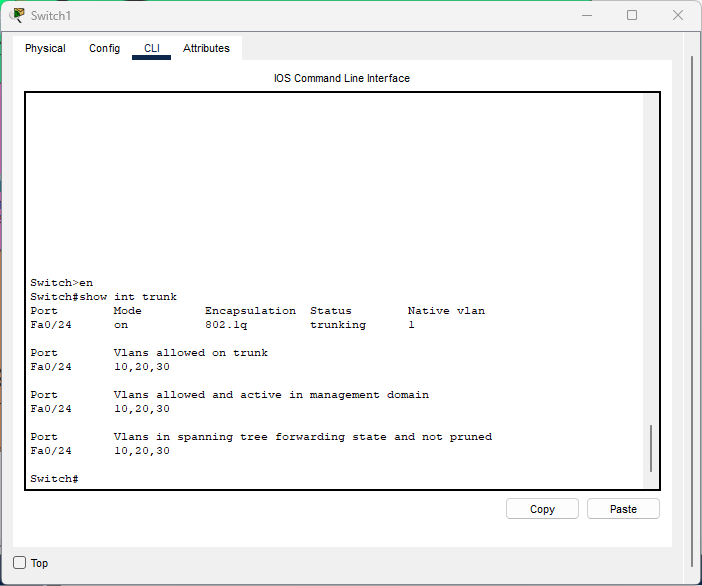
\includegraphics[width=0.6\textwidth]{img/tunksw1.png}
        \caption{Asignación de puestos en las VLANs Switch 1}
        \label{fig:swtru1}
    \end{figure}
    \begin{figure}[H]
        \centering
        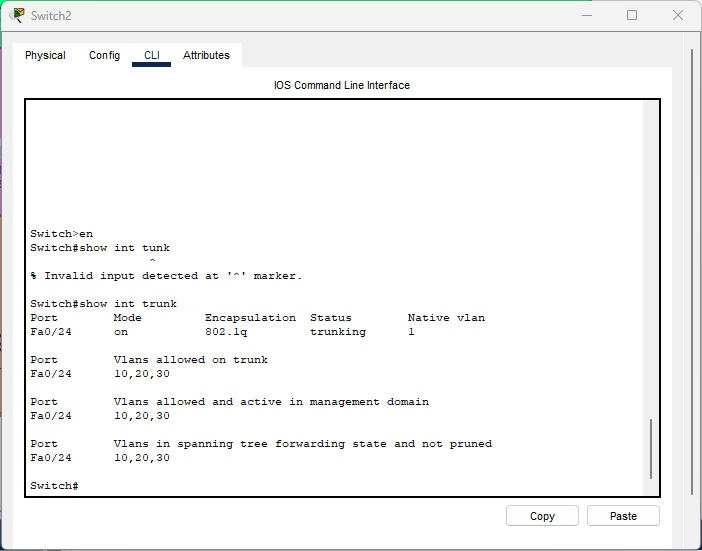
\includegraphics[width=0.6\textwidth]{img/trunksw2.png}
        \caption{Asignación de puestos en las VLANs Switch 2}
        \label{fig:swtru2}
    \end{figure}
    \begin{figure}[H]
        \centering
        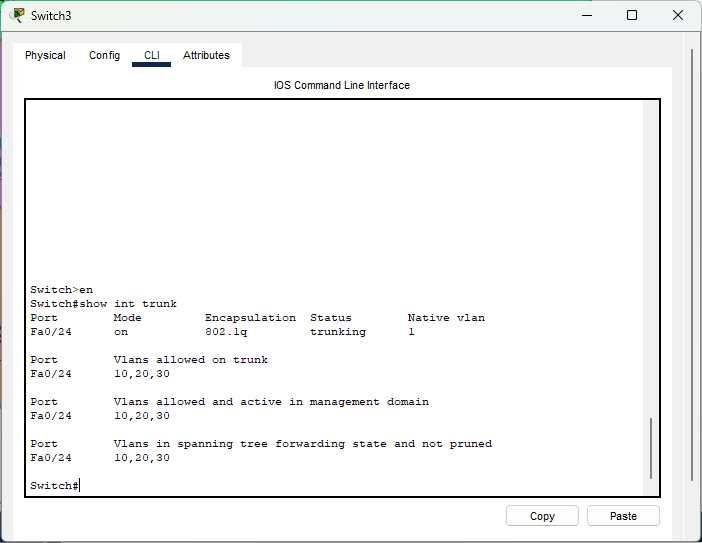
\includegraphics[width=0.6\textwidth]{img/trunk sw3.png}
        \caption{Asignación de puestos en las VLANs Switch 3}
        \label{fig:swtru3}
    \end{figure}
    \begin{figure}[H]
        \centering
        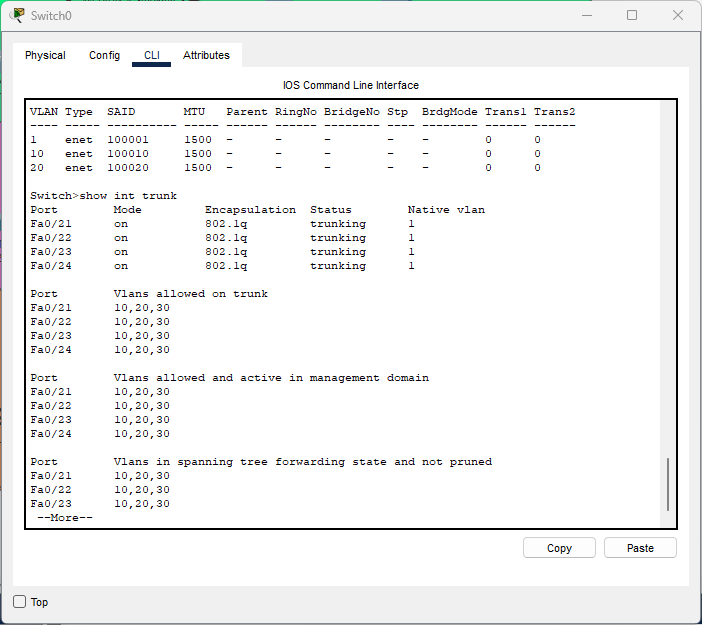
\includegraphics[width=0.6\textwidth]{img/trunsw4.png}
        \caption{Asignación de puestos en las VLANs Switch 3}
        \label{fig:swtru4}
    \end{figure}
    \subsection*{Configuración del router}
    Para la configuración del router, realizaremos dos acciones principales: primero, asignaremos las puertas de enlace; segundo, configuraremos los servidores DHCP, de manera que la red quede organizada de la siguiente forma:
    
    \begin{enumerate}
        \item [1] Asignación de las puertas de enlace y de los trunk:
        \begin{figure}[H]
            \centering
            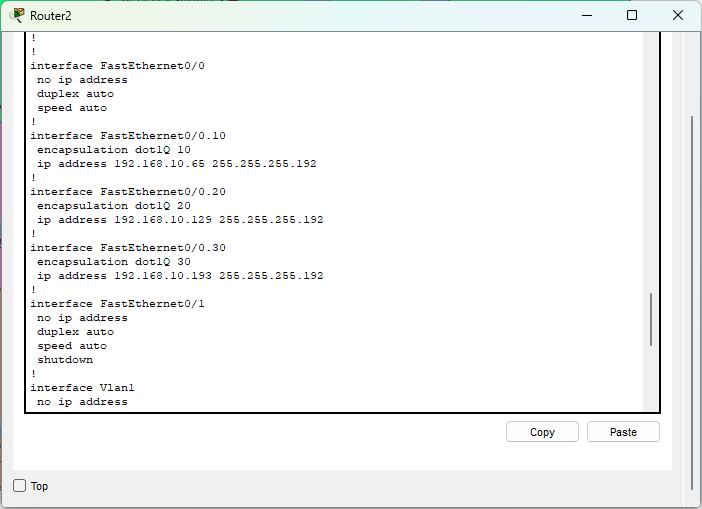
\includegraphics[width=0.6\textwidth]{img/Iprouter.png}
            \caption{Asignación de Puestas de enlace en el router}
            \label{fig:routerip}
        \end{figure}
        
        \item [2] Asignacion del DHCP en el servidor
        
        \begin{figure}[H]
            \centering
            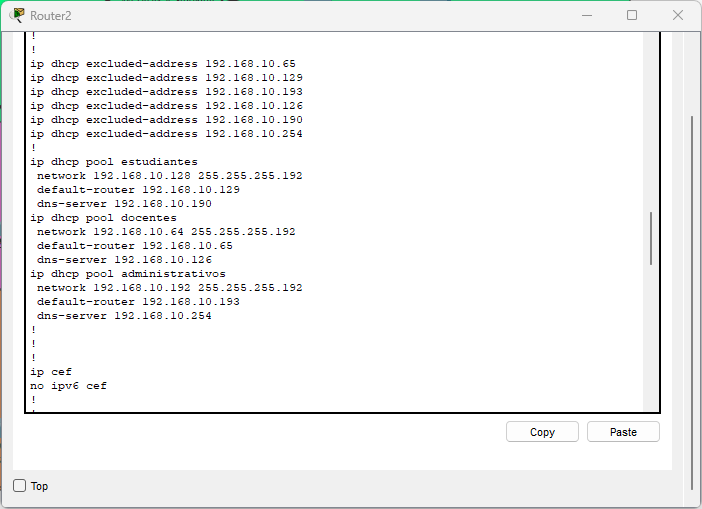
\includegraphics[width=0.6\textwidth]{img/dchpRouter.png}
            \caption{Asignación del DHCP en el router}
            \label{fig:routerDhcp}
        \end{figure}
        
        En la figura 15, podemos observar cómo se excluyen las direcciones IP necesarias para la red, como las correspondientes a las puertas de enlace y las direcciones de los servidores 
    \end{enumerate}
    \subsection*{Prueba del DHCP en los PCs}
    En esta sección, mostraremos cómo se asignan direcciones IP a los PCs mediante el protocolo DHCP.
    \begin{figure}[H]
        \centering
        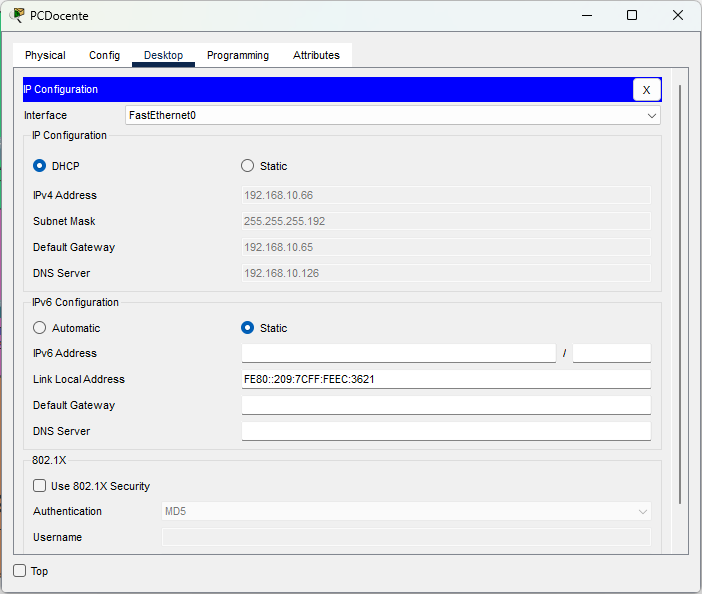
\includegraphics[width=0.6\textwidth]{img/dhcpdoc.png}
        \caption{Asignación del DHCP en el PC del docente}
        \label{fig:pcdDhcp}
    \end{figure}
    \begin{figure}[H]
        \centering
        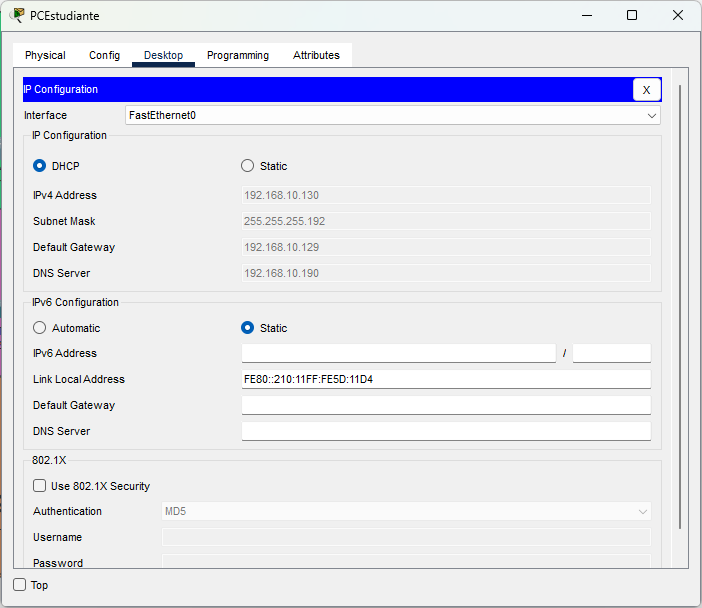
\includegraphics[width=0.6\textwidth]{img/dchpestu.png}
        \caption{Asignación del DHCP en el PC del Estudiante}
        \label{fig:pceDhcp}
    \end{figure}
    \begin{figure}[H]
        \centering
        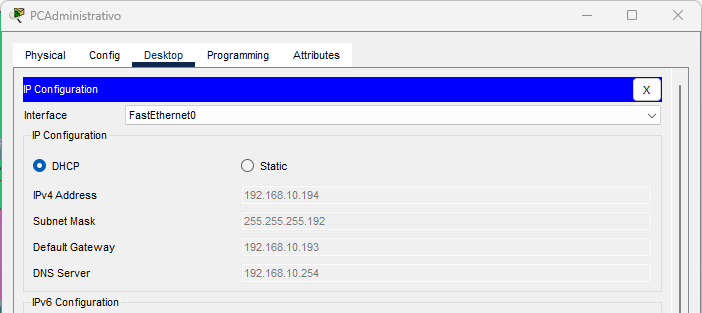
\includegraphics[width=0.6\textwidth]{img/dhcpAdminis.png}
        \caption{Asignación del DHCP en el PC del Administrativo}
        \label{fig:pcADhcp}
    \end{figure}
   
    \subsection*{Prueba del servicio web en los PCs}
    En esta sección, mostraremos cómo se muestran los servicios web en los PCs.
    \begin{figure}[H]
        \centering
        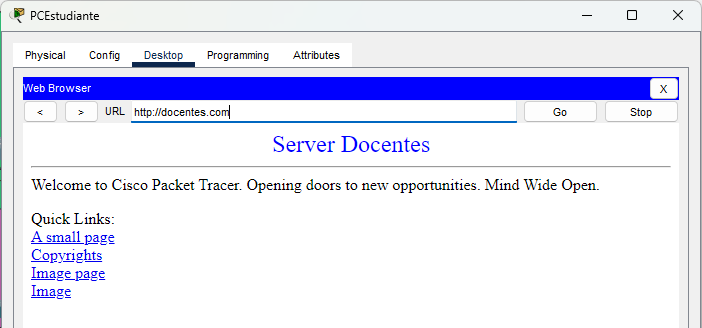
\includegraphics[width=0.6\textwidth]{img/wedDocEs.png}
        \caption{Asignación del servicio web del docente en el PC}
        \label{fig:pcdweb}
    \end{figure}
    \begin{figure}[H]
        \centering
        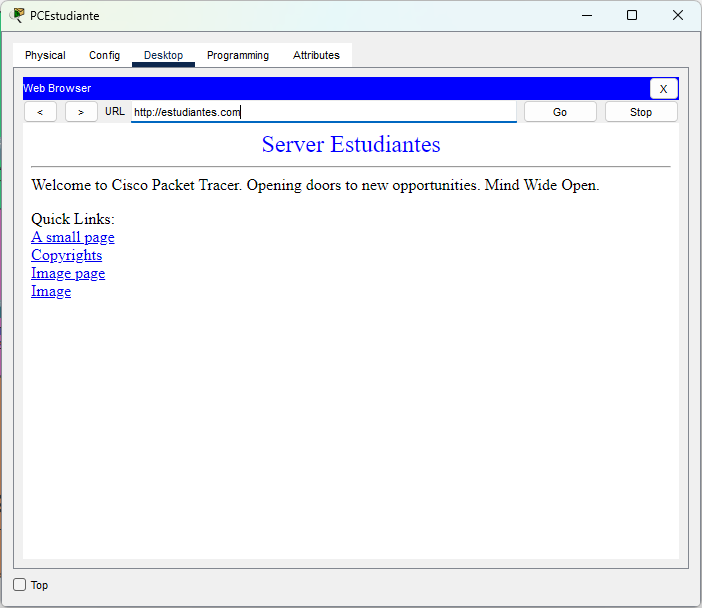
\includegraphics[width=0.6\textwidth]{img/web estudiantes.png}
        \caption{Asignación del servicio web del Estudiante en el PC}
        \label{fig:pceweb}
    \end{figure}
    \begin{figure}[H]
        \centering
        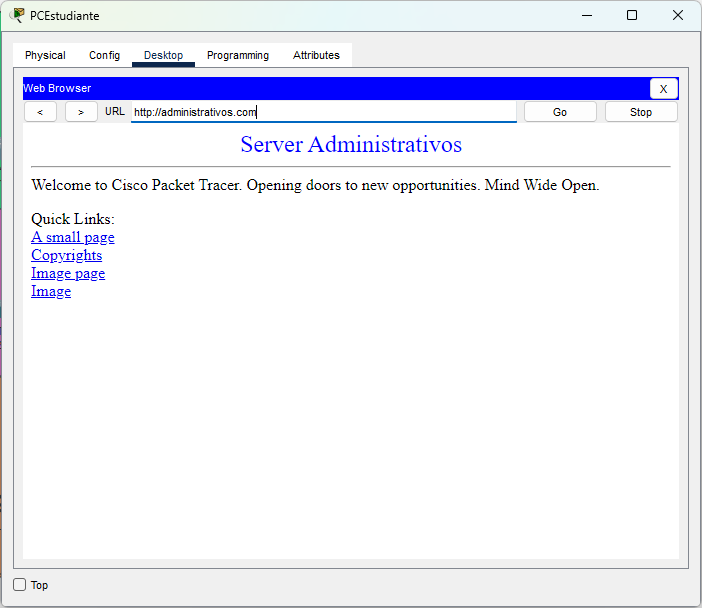
\includegraphics[width=0.6\textwidth]{img/web adminis.png}
        \caption{Asignación del servicio web del Administrativo en el PC}
        \label{fig:pcAweb}
    \end{figure}



\section{Conclusiones}
\textbf{Diego Moreno - 2243900185}

El proyecto logró diseñar e implementar una red institucional eficiente y segura, cumpliendo con los requerimientos del Instituto “Ing. Fátima Montserrat”. A través de técnicas de subnetting, VLANs y simulaciones, se optimizó la infraestructura, garantizando escalabilidad y rendimiento. Este ejercicio destacó la importancia de una planificación detallada y pruebas previas para minimizar errores en redes complejas.